\subsection{Interactive panel models}
\sourcepages{Lecture1-10.pdf, page 41, with the matrix intuition on page 40}
Consider the interactive panel model
\[
 Y_{it}=A_{i\cdot}B_{t\cdot}^{\mathsf T}+W_{it}\tau+\varepsilon_{it},
 \qquad\mathbb E[\varepsilon\mid A,B,W]=0,\tag{8.5}
\]
where $A\in\mathbb R^{n\times k}$, $B\in\mathbb R^{T\times k}$ and $k$ is a rank parameter. Equivalently,
\[
 Y_{it}=L_{it}+W_{it}\tau+\varepsilon_{it}
 \qquad\text{for a rank-$k$ matrix }L.
\]
\paragraph{My left-page matrix intuition.}
Place the $A$ values down the rows and the $B$ values across the columns. For rank one, their intersection has entry $a_i b_t$; for $k\ne1$, the entry is a sum $a_{i1}b_{t1}+a_{i2}b_{t2}+\cdots$. \begin{center}\begin{tikzpicture}[>=Stealth,font=\small]
\node at(0,2){$A$};\node at(3,3){$B$};
\node(a)at(0,0){$a_i$};\node(b)at(3,2){$b_t$};\node(p)at(3,0){$a_i b_t$};
\draw[->](a)--(p);\draw[->](b)--(p);
\node[align=center]at(3,-1){For $k>1$: $\sum_{j=1}^k a_{ij}b_{tj}$};
\end{tikzpicture}\end{center}

To handle this model, consider synthetic control and synthetic differences-in-differences. Suppose $W_{it}=1$ exactly when $i>n_0$ and $t>T_0$. The diagram partitions the outcome matrix at row $n_0$ and column $T_0$, with only the bottom-right block treated.
\begin{center}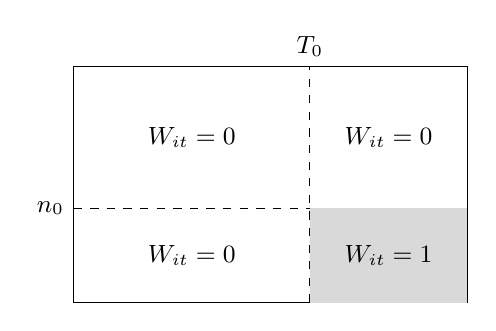
\begin{tikzpicture}[font=\small]
\draw(0,0)rectangle(5,3);\draw[dashed](3,0)--(3,3);\draw[dashed](0,1.2)--(5,1.2);
\fill[black!15](3,0)rectangle(5,1.2);
\node[above]at(3,3){$T_0$};\node[left]at(0,1.2){$n_0$};
\node at(4,.6){$W_{it}=1$};\node at(1.5,2.1){$W_{it}=0$};
\node at(4,2.1){$W_{it}=0$};\node at(1.5,.6){$W_{it}=0$};
\end{tikzpicture}\end{center}


Fit the untreated units to the pretreatment trajectory of the treated group:
\[
 \sum_{i=1}^{n_0}\gamma_iY_{it}
 \approx\alpha+\frac1{n-n_0}\sum_{i=n_0+1}^nY_{it},
 \qquad t=1,\ldots,T_0.
\]
\inkred{The first group is never treated; the second is treated after $T_0$.} The intercept $\alpha$ plays a role similar to a fixed effect. Choose weights by
\begin{align*}
 (\widehat\gamma,\widehat\alpha)\in
 \operatorname*{arg\,min}_{\gamma',\alpha}\quad&
 \left\|\sum_{i=1}^{n_0}\gamma'_iY_{i,1:T_0}
 -\frac1{n-n_0}\sum_{i=n_0+1}^nY_{i,1:T_0}
 -\alpha\mathbf1\right\|_2^2,\\
 \text{subject to}\quad&\sum_{i=1}^{n_0}\gamma'_i=1,
 \qquad\gamma'_i\ge0.\tag{8.7}
\end{align*}
\inkred{The purpose of $\gamma_i$ is to create parallel trends, so that the latent $A_i$ terms can be balanced.}

Finally, estimate the treatment coefficient in the weighted two-way model:
\[
 (\widehat\tau,\widehat\alpha,\widehat\beta)
 \in\operatorname*{arg\,min}_{\tau',\alpha',\beta'}
 \sum_{i,t}\gamma_i
 (Y_{it}-\alpha'_i-\beta'_t-W_{it}\tau')^2,\tag{8.8}
\]
where $\gamma_i=1/(n-n_0)$ for $i>n_0$.
\notearrow{red}{Treated-unit weights in the weighted regression (p.~41)}{\inkred{$\gamma_i=1/(n-n_0)$ for $i>n_0$.}}
 The closed-form treatment coefficient is
\begin{align*}
 \widehat\tau={}&\frac1{n-n_0}\sum_{i=n_0+1}^n
 \left\{\frac1{T-T_0}\sum_{t=T_0+1}^TY_{it}
 -\frac1{T_0}\sum_{t=1}^{T_0}Y_{it}\right\}\\
 &-\sum_{i=1}^{n_0}\gamma_i
 \left\{\frac1{T-T_0}\sum_{t=T_0+1}^TY_{it}
 -\frac1{T_0}\sum_{t=1}^{T_0}Y_{it}\right\}.
\end{align*}
\inkred{The red margin says this depends on $T_0$ and $n$.} Under an appropriate large-panel asymptotic regime, $n_0,n_1,T\to\infty$, the estimator is consistent. A further handwritten qualification below this statement is clipped by the bottom edge of the scan; the visible fragments refer to the specification in (8.5) and asymptotic normal inference, but a complete sentence cannot be recovered.
\begin{reviewnote}{qualification}{S1-033}{Latent-factor balance and panel asymptotics}{Lecture1-10.pdf, pp. 40, 41}
A close pretreatment fit alone does not prove that posttreatment counterfactual trends are balanced: preperiod factors must reveal the directions relevant after treatment, and noise/weight concentration must be controlled. The factorization has rank at most $k$; exact rank $k$ needs full-rank factors. The consistency claim is conditional on a suitable asymptotic regime and assumptions, not on $n,T\to\infty$ alone. The full synthetic-DID method may also use time weights and regularization. See \href{https://www.aeaweb.org/articles?id=10.1257/aer.20190159}{Arkhangelsky et al. (2021)} and lecture (8.7)--(8.9); the clipped handwriting is not reconstructed from that reference.
\end{reviewnote}


\paragraph{Left-page postscript.}
Synthetic control is not the only method for interactive fixed effects. For example, apply $k$-means clustering to the rows of the outcome matrix $Y$, then fit a time-varying baseline model separately for each group. A short reference is written as ``p66, literature'' [page number/reference unclear].

\subsection{Identification through exchangeability}
\sourcepages{Lecture1-10.pdf, page 43, with the extension on page 42}
Recall $Y_{it}=Y_{it}(0)+W_{it}\tau$. A design-based assumption is
\[
 Y_{i\cdot}(0)\perp W_{i\cdot}\mid S_i,
 \qquad S_i=\sum_{t=1}^TW_{it}.\tag{8.10}
\]
One implication: consider a linear estimator
\[
 \widehat\tau=\sum_{i,t}\gamma_{it}Y_{it},\tag{8.11}
\]
whose weight matrix depends only on $W$. Under (8.10), the untreated potential outcomes are exchangeable within a value of $S_i$, and
\[
 \mathbb E[\widehat\tau\mid W,\gamma]
 =\sum_{i,t}\gamma_{it}\mathbb E[Y_{it}(0)\mid S_i]
 +\tau\sum_{i,t}\gamma_{it}W_{it}.
\]
Thus unbiasedness follows if
\[
 \sum_{i,t}\gamma_{it}W_{it}=1,
 \qquad
 \sum_{i:S_i=s}\gamma_{it}=0
 \quad\text{for every }t\text{ and }s\in\mathcal S,
\]
where $\mathcal S$ is the support of $S_i$. \notearrow{red}{Within a stratum, the conditional expectation is constant (p.~43)}{$\sum_{i:S_i=s}\gamma_{it}=0$ removes $\sum_i\gamma_{it}E[Y_{it}(0)\mid S_i]$.}
\begin{reviewnote}{qualification}{S1-034}{Exchangeability across units and the variance criterion}{Lecture1-10.pdf, pp. 42, 43}
For the cancellation, require a common conditional mean $E[Y_{it}(0)\mid S_i=s]=m_t(s)$ across units, and conditions such as IID rows ensuring that conditioning on the full assignment matrix adds no information about a row beyond its own path. Within-row independence of $Y_i(0)$ and $W_i$ given $S_i$ alone does not impose cross-unit exchangeability. The combined restrictions give the claimed double robustness when feasible. Minimizing $\sum_{it}\gamma_{it}^2$ minimizes variance for conditionally uncorrelated homoskedastic cells; with within-unit covariance $\Sigma_i$, the variance criterion is $\sum_i\gamma_i'\Sigma_i\gamma_i$. Unbiasedness of feasible weights does not require that working variance model to be correct.
\end{reviewnote}


Choose $\gamma$ by minimizing variance under these unbiasedness constraints:
\begin{align*}
 \gamma\in\operatorname*{arg\,min}_{\gamma'}\quad&\sum_{i,t}(\gamma'_{it})^2,\\
 \text{subject to}\quad&\sum_{i,t}\gamma'_{it}W_{it}=1,
 \quad\sum_{i:S_i=s}\gamma'_{it}=0\quad\text{for all }s,t.\tag{8.14}
\end{align*}
\inkblue{Roughly, we need variation in $W_{it}$ among units with the same $S_i$.}

\paragraph{Left-page extension: two sets of identifying restrictions.}
Recall the two-way model
\[
 Y_{it}=\alpha_i+\beta_t+W_{it}\tau+\varepsilon_{it},
 \qquad\mathbb E[\varepsilon\mid\alpha,\beta,W]=0.\tag{8.2, recalled}
\]
The estimator (8.11) is also unbiased under this model if
\[
 \sum_t\gamma_{it}=0\ \text{for every }i,
 \qquad\sum_i\gamma_{it}=0\ \text{for every }t,
 \qquad\sum_{i,t}\gamma_{it}W_{it}=1.
\]
\inkred{The first two equalities cancel the fixed effects $\alpha_i$ and $\beta_t$, and the third normalizes the treatment coefficient.}

Combine the restrictions to obtain a doubly robust estimator: minimize $\sum_{i,t}\gamma_{it}^2$ subject to
\[
 \sum_{i,t}\gamma_{it}W_{it}=1,
 \qquad\sum_{i:S_i=s}\gamma_{it}=0\quad\text{for all }s,t,
\]
\[
 \sum_t\gamma_{it}=0\quad\text{for all }i,
 \qquad\sum_i\gamma_{it}=0\quad\text{for all }t.
\]
It is unbiased if either (8.2) or (8.10) holds. An abbreviated reference near the top of the supplement reads ``p67, [2019]'' [the citation is not fully identifiable from the scan].

\section{Lecture 9: Instrumental variables regression}
\sourcepages{Lecture1-10.pdf, page 45, with the three IV conditions on page 44}
Instrumental variables regression addresses endogenous treatment effects, where $Y_i(0)$ and $W_i$ are dependent.

\subsection{A structural model}
Start with a constant-effect model:
\[
 Y_i(w)=Y_i(0)+w\tau,\qquad Y_i=Y_i(W_i).\tag{9.1}
\]
Unconfoundedness ordinarily means $\{Y_i(w)\}\perp W_i$; in (9.1), this is $Y_i(0)\perp W_i$. Rewrite the model as
\notearrow{black}{Constant-effect potential outcomes and unconfoundedness (p.~45)}{$Y_i=\alpha+W_i\tau+\varepsilon_i$.}

\[
 Y_i=\alpha+W_i\tau+\varepsilon_i,\tag{9.2}
\]
where $\alpha=\mathbb E[Y_i(0)]$ and $\varepsilon_i=Y_i(0)-\mathbb E[Y_i(0)]$. Under unconfoundedness, $\mathbb E[\varepsilon_i\mid W_i]=0$, so OLS of $Y_i$ on $W_i$ estimates $\tau$.

With confounding, equation (9.2) still holds, but $\mathbb E[\varepsilon_i\mid W_i]\ne0$. OLS then targets
\begin{align*}
 \tau_{\mathrm{OLS}}
 &=\frac{\operatorname{Cov}(Y_i,W_i)}{\operatorname{Var}(W_i)}\\
 &=\frac{\operatorname{Cov}(\tau W_i+\varepsilon_i,W_i)}{\operatorname{Var}(W_i)}
 =\tau+\frac{\operatorname{Cov}(\varepsilon_i,W_i)}{\operatorname{Var}(W_i)}
 \ne\tau.
\end{align*}
\inkred{The ratio is underlined as the OLS coefficient.}
\begin{reviewnote}{qualification}{S1-035}{Dependence need not create a nonzero linear bias}{Lecture1-10.pdf, pp. 45}
The exact identity $\tau_{\rm OLS}=\tau+\operatorname{Cov}(\varepsilon,W)/\operatorname{Var}(W)$ is correct. However, dependence of $Y(0)$ and $W$ does not necessarily imply nonzero conditional mean or nonzero covariance. For example, $Y(0)$ can have treatment-dependent variance but the same conditional mean. The displayed $\ne\tau$ describes the confounded case with nonzero covariance, not a consequence of every dependence. Identification by the subsequent IV ratio requires its nonzero denominator.
\end{reviewnote}


\subsection{Identification with an instrument}
Introduce $Z_i$:
\[
 Y_i=\alpha+W_i\tau+\varepsilon_i,\qquad\varepsilon_i\perp Z_i,
 \qquad W_i=Z_i\gamma+\eta_i.\tag{9.4}
\]
Since $Z_i$ is uncorrelated with $\varepsilon_i$,
\[
 \operatorname{Cov}(Y_i,Z_i)
 =\operatorname{Cov}(\tau W_i+\varepsilon_i,Z_i)
 =\tau\operatorname{Cov}(W_i,Z_i).
\]
Hence
\[
 \tau=\frac{\operatorname{Cov}(Y_i,Z_i)}{\operatorname{Cov}(W_i,Z_i)},
 \qquad
 \widehat\tau=\frac{\widehat{\operatorname{Cov}}(Y_i,Z_i)}
 {\widehat{\operatorname{Cov}}(W_i,Z_i)}.
\]

\paragraph{My left-page checklist for an IV.}
\begin{enumerate}
 \item \textbf{Exogenous:} $\varepsilon_i\perp Z_i$.
 \item \textbf{Relevant:} $\operatorname{Cov}(W_i,Z_i)\ne0$.
 \item \textbf{Exclusion restriction:} every effect of $Z_i$ on $Y_i$ must pass through $W_i$.
\end{enumerate}
\begin{center}\begin{tikzpicture}[>=Stealth,font=\small]
\node(z)at(0,0){$Z_i$};\node(w)at(2,0){$W_i$};\node(y)at(4,0){$Y_i$};
\draw[->,red](z)--(w);\draw[->,red](w)--(y);
\draw[->](w) to[bend right=45]node[below]{other treatment pathways}(y);
\end{tikzpicture}\end{center}

\subsection{Optimal instruments}
\sourcepages{Lecture1-10.pdf, page 47, with extensions on page 46 and the estimating-equation reminder on page 48}
Allow a high-dimensional instrument $Z_i\in\mathcal Z$:
\[
 Y_i=\tau W_i+\varepsilon_i,\qquad\varepsilon_i\perp Z_i,
 \qquad Y_i,W_i\in\mathbb R.
\]
For a function $w:\mathcal Z\to\mathbb R$,
\[
 \tau=\frac{\operatorname{Cov}(Y_i,w(Z_i))}
 {\operatorname{Cov}(W_i,w(Z_i))},\tag{9.8}
\]
with nonzero denominator. Which transformation $w(\cdot)$ is optimal? The estimator is
\begin{align*}
 \widehat\tau_w
 &=\frac{\widehat{\operatorname{Cov}}(Y_i,w(Z_i))}
 {\widehat{\operatorname{Cov}}(W_i,w(Z_i))}\\
 &=\frac{n^{-1}\sum_i(Y_i-\overline Y)(w(Z_i)-\overline{w(Z)})}
 {n^{-1}\sum_i(W_i-\overline W)(w(Z_i)-\overline{w(Z)})},\tag{9.9}
\end{align*}
where $\overline Y=n^{-1}\sum_iY_i$, with analogous definitions for the other averages. It solves the estimating equation
\[
 \frac1n\sum_i(w(Z_i)-\overline{w(Z)})
 \{Y_i-\overline Y-\widehat\tau_w(W_i-\overline W)\}=0.\tag{9.10}
\]
The source writes
\[
 n(\widehat\tau_w-\tau)\Rightarrow\mathcal N(0,V_w),
 \qquad
 V_w=\frac{\operatorname{Var}(\varepsilon_i)\operatorname{Var}(w(Z_i))}
 {\operatorname{Cov}(W_i,w(Z_i))^2}.\tag{9.11, source scaling}
\]
\begin{reviewnote}{original}{S1-036}{The IV normal limit uses square-root-n scaling}{Lecture1-10.pdf, pp. 47, 48}
The correct limit is $\sqrt n(\widehat\tau_w-\tau)\Rightarrow N(0,V_w)$. The first-order expansion is
\[
\sqrt n(\widehat\tau_w-\tau)=
\frac{n^{-1/2}\sum_i(w(Z_i)-E[w(Z)])\varepsilon_i}
{\operatorname{Cov}(W,w(Z))}+o_p(1),
\]
with centered errors, IID observations, finite required moments and a nonzero limiting covariance. This gives the displayed $V_w$ under $\varepsilon\perp Z$. Compare official lecture (9.12); its equation numbering differs from the handwritten notes.
\end{reviewnote}



Because $Z_i\perp\varepsilon_i$ and $\mathbb E[\varepsilon_i]=0$,
\[
 \operatorname{Var}\{\varepsilon_i(w(Z_i)-\mathbb E[w(Z_i)])\}
 =\operatorname{Var}(\varepsilon_i)\operatorname{Var}(w(Z_i)).
\]
The optimization written in the notebook is
\notearrow{red}{Use the reciprocal of the variance-dependent ratio (p.~47)}{The source optimization for $w^*(\cdot)$ below.}

\[
 w^*(\cdot)\in\operatorname*{arg\,min}_{w'}
 \frac{\operatorname{Cov}(W_i,w'(Z_i))^2}{\operatorname{Var}(w'(Z_i))}.
\]
Its stated solution is
\[
 w^*(z)\propto\mathbb E[W_i\mid Z_i=z].
\]
\notearrow{red}{$w^*(z)\propto E[W_i\mid Z_i=z]$ (p.~47)}{\inkred{The best prediction of $W_i$ from $Z_i$.}}
\begin{reviewnote}{original}{S1-037}{Maximize the covariance ratio}{Lecture1-10.pdf, pp. 47}
Minimizing $V_w$ requires
\[
\arg\max_w\frac{\operatorname{Cov}(W,w(Z))^2}{\operatorname{Var}(w(Z))}.
\]
Writing $m(Z)=E[W\mid Z]$, conditional expectation and Cauchy--Schwarz give $\operatorname{Cov}(W,w)^2=\operatorname{Cov}(m,w)^2\le\operatorname{Var}(m)\operatorname{Var}(w)$. Equality holds for $w=a+bm$, $b\ne0$, provided $\operatorname{Var}(m)>0$. Thus the prediction intuition is correct; the optimization direction is not. The result uses the source's independence/homoskedastic-instrument setup; it is not the general heteroskedastic optimal-instrument formula. See official lecture (9.13)--(9.15).
\end{reviewnote}



\paragraph{Left-page extension: conditioning on covariates.}
\begin{inkblock}{red}
The condition can be extended to $\varepsilon_i\perp Z_i\mid X_i$, giving
\[
 \tau(x)=\frac{\operatorname{Cov}(Y_i,w(Z_i)\mid X_i=x)}
 {\operatorname{Cov}(W_i,w(Z_i)\mid X_i=x)}.
\]
The annotation mentions a doubly robust estimator of the average effect $\tau=\mathbb E[\tau(X)]$, and a random-forest estimator of $\tau(\cdot)$.
\end{inkblock}

\begin{reviewnote}{qualification}{S1-038}{What the conditional IV ratio identifies}{Lecture1-10.pdf, pp. 46}
The ratio equals $\tau(x)$ under a conditional structural model $Y=a(X)+W\tau(X)+\varepsilon$ with $E[\varepsilon\mid Z,X]=0$ and nonzero conditional first-stage covariance. Under unrestricted individual treatment heterogeneity, conditional exogeneity of the instrument alone does not make this ratio the general CATE; with appropriate monotonicity it may instead identify a conditional local effect. A doubly robust estimator or forest must target the identified effect under its particular assumptions.
\end{reviewnote}


Another reminder on the same page: for independent $X_1,X_2$,
\begin{align*}
 \operatorname{Var}(X_1X_2)
 ={}&\operatorname{Var}(X_1)\operatorname{Var}(X_2)\\
 &+\mathbb E[X_2]^2\operatorname{Var}(X_1)
 +\mathbb E[X_1]^2\operatorname{Var}(X_2).
\end{align*}

\paragraph{Starred supplement: estimating equations and the delta method.}
If functions $\psi_i$ satisfy $\mathbb E[\psi_i(\theta)]=0$, and $\widehat\theta$ is estimated by
\[
 \frac1n\sum_{i=1}^n\psi_i(\widehat\theta)=0,
\]
then, in the regular setting described by the note's nonparametric delta-method reminder,
\[
 \sqrt n(\widehat\theta-\theta)\Rightarrow\mathcal N(0,V),
 \qquad
 V=\frac{\operatorname{Var}(\psi_i(\theta))}
 {\mathbb E[\psi_i'(\theta)]^2}.
\]

\subsection{Cross-fitting and feasible estimation}
\sourcepages{Lecture1-10.pdf, page 49}
The optimal instrument is $w^*(z)=\mathbb E[W_i\mid Z_i=z]$. The general procedure is:
\begin{enumerate}
 \item Fit a nonparametric first-stage regression to estimate $\mathbb E[W_i\mid Z_i=z]$, obtaining $\widehat w(\cdot)$.
 \item Use $\widehat w(\cdot)$ as the instrument in (9.9), obtaining $\widehat\tau_w$.
\end{enumerate}
However, with many instruments this can create overfitting bias. If $\widehat w(Z_i)$ is fit using the entire data set, it need not be independent of $\varepsilon_i$: the fitted instrument can inherit the dependence of $W_i$ on $\varepsilon_i$.

\paragraph{My blue example in the margin.}
\begin{inkblock}{blue}
Suppose $Z_i$ is noise. The note writes
\[
 W_i=\alpha+\beta Z_i+\eta_i,
 \qquad Y_i=\gamma+\delta\widehat W_i+\varepsilon_i
 =\gamma+\delta(\widehat\alpha+\widehat\beta Z_i)+\varepsilon_i,
\]
marks the fitted term as biased, and draws an arrow comparing it to $Y_i=\gamma+\delta W_i+\varepsilon_i$.
\notearrow{blue}{Fitted-treatment equation in the blue example (p.~49)}{$Y_i=\gamma+\delta W_i+\varepsilon_i$; ``equivalent'' in the source.}
 The point of the annotation is that using an overfit first stage does not remove the problematic dependence.
\end{inkblock}

\begin{reviewnote}{original}{S1-039}{Substituting a fitted treatment changes the structural residual}{Lecture1-10.pdf, pp. 49}
From $Y=\gamma+\delta W+\varepsilon$ one obtains
\[
Y=\gamma+\delta\widehat W+\{\varepsilon+\delta(W-\widehat W)\}.
\]
The same $\varepsilon$ cannot generally be retained unless $\delta(W-\widehat W)=0$. The author's warning about first-stage overfitting is sound, but the displayed equivalence needs this changed residual. If $Z$ is pure noise, relevance fails; cross-fitting prevents reuse of an observation's noise but does not create a relevant instrument.
\end{reviewnote}


Use $K$-fold cross-fitting instead. With $k(i)$ the fold containing observation $i$,
\[
 \widehat\tau=
 \frac{\widehat{\operatorname{Cov}}(Y_i,\widehat w^{(-k(i))}(Z_i))}
 {\widehat{\operatorname{Cov}}(W_i,\widehat w^{(-k(i))}(Z_i))}.\tag{9.13}
\]
The corresponding fitted instrument is independent of the observation's error under the stated sampling setup. In particular, if $\widehat w^{(-k(i))}(z)$ is mean-square consistent for $\mathbb E[W_i\mid Z_i=z]$, then (9.13) is asymptotically equivalent to the oracle version of (9.9). The red reminder writes this consistency as
\begin{inkblock}{red}
\[
 \lim_{n\to\infty}\mathbb E[(\widehat w_n-\mathbb E[W\mid Z])^2]=0,
\]
\end{inkblock}
\inkred{where $n$ is the sample size.}
\begin{reviewnote}{qualification}{S1-040}{Cross-fitted IV still needs a nonvanishing first stage}{Lecture1-10.pdf, pp. 49}
With independent observations, a fixed number of folds, suitable moments, and $\operatorname{Var}(E[W\mid Z])>0$ bounded away from zero, mean-square-consistent first-stage prediction can emulate the oracle at first order. Training outside the observation's fold removes own-observation dependence under $\varepsilon\perp Z$. It does not justify normal inference when instruments become weak, nor independence across all fitted observations (their training sets overlap).
\end{reviewnote}


\subsection{Nonparametric instrumental variables regression}
\sourcepages{Lecture1-10.pdf, page 50}
The previous model assumed $Y_i=W_i\tau+\varepsilon_i$. The handwritten parenthesis says ``$Z_i$ acts linearly on $Y_i$.''
\begin{reviewnote}{original}{S1-041}{The linear structural coefficient multiplies treatment}{Lecture1-10.pdf, pp. 50}
The constant structural effect is linear in $W_i$, not necessarily in $Z_i$. The instrument may influence treatment nonlinearly. The subsequent generalization replaces $W_i\tau$ by $g(W_i)$; that formula correctly describes the intended extension.
\end{reviewnote}
 Generalize it to
\[
 Y_i=g(W_i)+\varepsilon_i,\qquad Z_i\perp\varepsilon_i,
 \qquad Y_i,W_i\in\mathbb R,\quad Z_i\in\mathcal Z,
\]
where $g$ is a general smooth function. \begin{inkblock}{blue}
\textbf{Blue warning:} we cannot simply run a nonparametric regression of $Y_i$ on $W_i$, because
\[
 g(w)\ne\mathbb E[Y_i\mid W_i=w].
\]
\end{inkblock}



Since $Z_i\perp\varepsilon_i$ and $\mathbb E[\varepsilon_i]=0$,
\begin{align*}
 \mathbb E[Y_i\mid Z_i=z]
 &=\mathbb E[g(W_i)+\varepsilon_i\mid Z_i=z]\\
 &=\mathbb E[g(W_i)\mid Z_i=z]
 =\int_{\mathbb R}g(w)f(w\mid z)\,dw.\tag{9.15}
\end{align*}
Here $f(w\mid z)$ is the conditional density of $W_i$ given $Z_i=z$.

A learning procedure:
\begin{enumerate}
 \item Estimate $\widehat f(w\mid z)$ using cross-fitting.
 \item Choose a suitable function class $\mathcal G$ and minimize the loss to estimate $g$:
 \[
 \widehat g\in\operatorname*{arg\,min}_{g\in\mathcal G}
 \frac1n\sum_{i=1}^n\left\{
 Y_i-\int_{\mathbb R}g(w)\widehat f^{(-k(i))}(w\mid Z_i)\,dw
 \right\}^{\!2}.\tag{9.16}
 \]
\end{enumerate}
To solve this in practice, approximate $g$ with a basis expansion,
\[
 g_K(w)=\sum_{k=1}^K\beta_k\psi_k(w),
\]
where the $\psi_k$ are predetermined basis functions. As $K$ grows, $g_K$ better approximates $g$. Then
\[
 \widehat\beta\in\operatorname*{arg\,min}_\beta
 \frac1n\sum_{i=1}^n
 \{Y_i-\widehat m^{(-k(i))}(Z_i)^{\mathsf T}\beta\}^2,\tag{9.17}
\]
with components
\[
 \widehat m_k^{(-k(i))}(Z_i)=
 \int_{\mathbb R}\psi_k(w)\widehat f^{(-k(i))}(w\mid Z_i)\,dw.
\]
\inkblue{\textbf{Bottom-margin interpretation:} consistency for $g(\cdot)$ needs conditions; (9.15) is complicated, while (9.17) turns the problem into regression by minimizing the loss for each basis coefficient.} \inkblue{The blue margin adds that using (9.17) comes at the cost of regularization.} The remaining bottom-edge wording is clipped and cannot be fully read. A nearby note says ``analogous to 9.13.''
\begin{reviewnote}{qualification}{S1-042}{NPIV identification and inverse-problem regularization}{Lecture1-10.pdf, pp. 50}
Let $(Th)(z)=E[h(W)\mid Z=z]$. The moment equation identifies $g$ only if $T$ is injective on the chosen function class: $E[h(W)\mid Z]=0$ implies $h(W)=0$ almost surely (a completeness condition). Even then inversion may be ill posed, so accurate first-stage density estimates alone do not ensure accurate recovery of $g$. Sieve dimension or other regularization must control this instability and approximation error. Also, $E[Y\mid W=w]=g(w)+E[\varepsilon\mid W=w]$; inequality with $g(w)$ holds when that conditional error mean is nonzero. See \href{https://doi.org/10.1111/1468-0262.00459}{Newey and Powell (2003)}, which characterizes identification through completeness and develops regularized series estimation.
\end{reviewnote}


\section{Lecture 10: Local average treatment effects}
\sourcepages{Lecture1-10.pdf, page 52, then the compliance table and derivation on page 51}
Recall the Lecture 9 IV model:
\[
 Y_i=\alpha+W_i\tau+\varepsilon_i,\quad\varepsilon_i\perp Z_i,
 \qquad W_i=Z_i\gamma+\eta_i.\tag{10.1}
\]
When $Z_i$ is binary,
\begin{align*}
 \tau&=\frac{\operatorname{Cov}(Y_i,Z_i)}{\operatorname{Cov}(W_i,Z_i)}\\
 &=\frac{\mathbb E[Y_i\mid Z_i=1]-\mathbb E[Y_i\mid Z_i=0]}
 {\mathbb E[W_i\mid Z_i=1]-\mathbb E[W_i\mid Z_i=0]}.\tag{10.2}
\end{align*}

\subsection{Treatment effects under noncompliance}
In an RCT with noncompliance, $Y_i\in\mathbb R$ is the ordinary outcome; \inkred{$W_i\in\{0,1\}$ is the treatment actually received} and is not randomized; \inkred{$Z_i\in\{0,1\}$ is randomized treatment assignment.}

The constant $\tau$ in (10.1) may not be appropriate, and treatment receipt may be related to the treatment effect. Define potential treatment receipt $W_i(0),W_i(1)$, with $W_i=W_i(Z_i)$ and $Y_i=Y_i(W_i(Z_i))$.

The IV validity assumptions are:
\begin{itemize}
 \item \textbf{Exclusion restriction:} $Y_i(w,z)=Y_i(w)$. Assignment affects the outcome only through treatment receipt.
 \item \textbf{Exogeneity:} $\{Y_i(0),Y_i(1),W_i(0),W_i(1)\}\perp Z_i$. Assignment is randomized.
 \item \textbf{Relevance:} $\mathbb E[W_i(1)-W_i(0)]\ne0$. Assignment affects treatment receipt.
\end{itemize}

There are four compliance types:
\begin{center}
\begin{tabular}{lcc}
 & $W_i(1)=0$ & $W_i(1)=1$\\\hline
 $W_i(0)=0$ & Never-taker & Complier\\
 $W_i(0)=1$ & Defier & Always-taker
\end{tabular}
\end{center}
Assume there are no defiers, that is, \textbf{monotonicity}:
\begin{inkblock}{red}
\[
 W_i(1)\ge W_i(0)\quad\text{for every }i.
\]
\end{inkblock}
Then
\begin{align*}
 &\mathbb E[Y_i\mid Z_i=1]-\mathbb E[Y_i\mid Z_i=0]\\
 &\quad=\mathbb E[Y_i(W_i(1))\mid Z_i=1]
 -\mathbb E[Y_i(W_i(0))\mid Z_i=0]\\
 &\quad=\mathbb E[Y_i(W_i(1))-Y_i(W_i(0))]\\
 &\quad=\mathbb E[\mathbf1\{C_i=\mathrm{complier}\}
 (Y_i(1)-Y_i(0))].
\end{align*}
If compliers exist, applying Bayes' rule gives
\begin{align*}
 \tau_{\mathrm{LATE}}
 &=\frac{\mathbb E[Y_i\mid Z_i=1]-\mathbb E[Y_i\mid Z_i=0]}
 {\mathbb E[W_i\mid Z_i=1]-\mathbb E[W_i\mid Z_i=0]}\\
 &=\mathbb E[Y_i(1)-Y_i(0)\mid C_i=\mathrm{complier}].\tag{10.3}
\end{align*}
\inkblue{This is the complier average treatment effect.}
\begin{reviewnote}{qualification}{S1-043}{LATE, ATE, and individual contrasts}{Lecture1-10.pdf, pp. 51, 52}
The derivation also requires $0<P(Z=1)<1$ and a positive complier share. Under the stated exclusion, exogeneity and monotonicity, the Wald ratio identifies the complier average effect, not the population ATE in general. The blue expression $E[Y(1)-Y(0)]$ is an ATE; an individual effect is $Y_i(1)-Y_i(0)$. The marginal label itself remains ambiguous. The author's point that never-takers reveal no treated outcome is correct.
\end{reviewnote}


\paragraph{My blue postscript.}
\begin{inkblock}{blue}
When the constant-effect model (10.1) fails and there are never-takers, always-takers, defiers, and so on, the individual contrast $Y_i(1)-Y_i(0)$ is not generally observable. In particular, a never-taker is never observed with $W_i=1$. The marginal line writes an ``IATE'' expression as $\mathbb E[Y_i(1)-Y_i(0)]$ [the label and intended distinction between individual and average effects are not resolved in the scan].
\end{inkblock}


\subsection{Supply and demand}
\sourcepages{Lecture1-10.pdf, page 53}
For each market $i=1,\ldots,n$, let $S_i(p,z)$ be its supply curve and $Q_i(p,z)$ its demand curve, where price $p\in\mathbb R$ and the instrument $z\in\{0,1\}$. Assume supply is continuous and increasing in price, while demand is continuous and decreasing. The equilibrium price $P_i$ is the unique solution to
\[
 S_i(P_i,Z_i)=Q_i(P_i,Z_i).
\]
Thus $Z_i$ is the IV, $P_i$ is treatment, and $Q_i(P_i,Z_i)$ is the outcome $Y_i$. \begin{inkblock}{red}\[ Z_i\longrightarrow S_i\longrightarrow P_i\longrightarrow Q_i(P_i). \]\end{inkblock}

Conditions:
\begin{itemize}
 \item Exclusion: $Q_i(p,z)=Q_i(p)$ for every $p,z$.
 \item Exogeneity: $\{Q_i(p),S_i(p,z)\}\perp Z_i$.
 \item Relevance: $\operatorname{Cov}(P_i,Z_i)\ne0$.
 \item Monotonicity: $S_i(p,1)\le S_i(p,0)$ for all relevant $p$ [the source writes the equilibrium-price symbol in this condition].
\end{itemize}
If $Q_i(p)$ is differentiable, let $Q_i'(p)$ denote its derivative. The author's parenthetical qualification says that ordinary differentiability is not necessary: because $Q_i(\cdot)$ is monotone decreasing, a derivative in the distributional sense exists.
\begin{align*}
 \tau_{\mathrm{LATE}}
 &=\frac{\mathbb E[Q_i\mid Z_i=1]-\mathbb E[Q_i\mid Z_i=0]}
 {\mathbb E[P_i\mid Z_i=1]-\mathbb E[P_i\mid Z_i=0]}\\
 &=\frac{\displaystyle\int
 \mathbb E[Q_i'(p)\mid P_i(0)\le p\le P_i(1)]
 P[P_i(0)\le p\le P_i(1)]\,dp}
 {\displaystyle\int P[P_i(0)\le p\le P_i(1)]\,dp}.
\end{align*}
\inkred{The denominator is annotated ``total integral.''}
\begin{reviewnote}{qualification}{S1-044}{Supply-demand existence and the derivative representation}{Lecture1-10.pdf, pp. 53}
Continuity and opposing strict slopes give at most one intersection; existence also requires that the curves cross. The supply shift must hold at every relevant price to imply $P_i(1)\ge P_i(0)$. The displayed ordinary integral with $Q_i'(p)\,dp$ is valid when demand is absolutely continuous over the affected price intervals and integrable enough to interchange expectation and integration. A monotone continuous demand curve can have a singular continuous component, so a distributional derivative must instead be treated as a signed measure $dQ_i(p)$. Then use $Q_i(P_i(1))-Q_i(P_i(0))=\int_{(P_i(0),P_i(1)]}dQ_i$. The author's distributional-derivative idea is valid with this measure interpretation, not as an ordinary density in all cases.
\end{reviewnote}


\paragraph{Derivation in the notebook.}
\begin{align*}
 &\mathbb E[Q_i\mid Z_i=1]-\mathbb E[Q_i\mid Z_i=0]\\
 &\quad=\mathbb E[Q_i(P_i(1))\mid Z_i=1]
 -\mathbb E[Q_i(P_i(0))\mid Z_i=0]\\
 &\quad=\mathbb E[Q_i(P_i(1))-Q_i(P_i(0))]\\
 &\quad=\mathbb E\left[\int_{P_i(0)}^{P_i(1)}Q_i'(p)\,dp\right]\\
 &\quad=\int\mathbb E[Q_i'(p)\mid P_i(0)\le p\le P_i(1)]
 P[P_i(0)\le p\le P_i(1)]\,dp.
\end{align*}
\notearrow{red}{Fubini: interchange integration order (p.~53)}{$E[\int Q_i'(p)\,dp]$ becomes an integral of the expectation.}

\subsection{Threshold crossing and willingness to pay}
\sourcepages{Lecture1-10.pdf, page 55, with the diagram and decomposition on page 54}
Suppose each subject has an unobserved endogenous variable $U_i$ such that
\[
 W_i=\mathbf1\{U_i\ge c(Z_i)\},
\]
where $c(z)$ is a cutoff function depending on the instrument. Without loss of generality, take $U_i\sim\operatorname{Unif}[0,1]$, giving
\[
 c(z)=1-P(W_i=1\mid Z_i=z).
\]
\begin{reviewnote}{qualification}{S1-046}{Uniform normalization and cutoff support}{Lecture1-10.pdf, pp. 55}
The identity $c(z)=1-P(W=1\mid Z=z)$ uses $U\perp Z$, $U\sim\mathrm{Unif}[0,1]$ and an effective cutoff in $[0,1]$. Uniform normalization follows directly from a continuous latent CDF (with a suitable monotone reparameterization); atoms need additional care, such as a randomized latent rank. These are assumptions/normalizations of the threshold model, not a consequence of the indicator rule alone.
\end{reviewnote}

The IV setup imposes:
\begin{enumerate}
 \item Potential outcomes $Y_i(0),Y_i(1)$ with $Y_i=Y_i(W_i)$: \inkblue{the instrument has no direct route to the outcome.}
 \item $\{Y_i(0),Y_i(1),U_i\}\perp Z_i$: \inkblue{exogeneity.}
 \item $c(Z_i)$ has a nontrivial distribution: \inkblue{relevance.}
 \item $c(z)$ is c\`adl\`ag (right-continuous with left limits) and nondecreasing. \inkblue{The margin says that $W_i$ is nondecreasing in $Z_i$.}
\begin{reviewnote}{original}{S1-045}{Increasing cutoffs decrease treatment receipt}{Lecture1-10.pdf, pp. 55, 57}
For fixed $U_i$, $W_i(z)=\mathbf1\{U_i\ge c(z)\}$ is nonincreasing when $c$ is nondecreasing. The single-jump middle group therefore switches from treated to untreated as $z$ increases. Relative to the earlier increasing-treatment instrument convention it is the opposite switching direction; it can be called a complier group after reversing the instrument orientation. Both IV covariances change sign together, so the positive-weight treatment-effect interpretation still holds. This convention issue does not invalidate the IV ratio.
\end{reviewnote}

\end{enumerate}


Define the marginal treatment effect (MTE)
\[
 \tau(u)=\mathbb E[Y_i(1)-Y_i(0)\mid U_i=u].\tag{10.6}
\]
The IV estimand is a weighted average of $\tau(u)$. In the notes, $Z_i\sim\mathcal N(0,1)$, with density $\varphi$. Let $S\subset\mathbb R$ be the discontinuity set of $c$, and
\[
 c_-(z)=\lim_{a\uparrow z}c(a).
\]
The displayed representation is
\[
 \tau_{\mathrm{LATE}}=
 \frac{\displaystyle\sum_{z\in S}
 \left\{\int_{c_-(z)}^{c(z)}\tau(u)\,du\right\}\varphi(z)
 +\int_{\mathbb R\setminus S}\tau(c(z))c'(z)\varphi(z)\,dz}
 {\displaystyle\sum_{z\in S}(c(z)-c_-(z))\varphi(z)
 +\int_{\mathbb R\setminus S}c'(z)\varphi(z)\,dz}.
\]
This displays the IV estimand as a convex average of marginal treatment effects.

\paragraph{My left-page explanation of the weights.}
The drawing plots $c(z)$ against $z$ with an open dot at the left limit and a filled dot at the value after a jump. The jump location belongs to $S$.
\begin{center}\begin{tikzpicture}[>=Stealth,font=\small,x=1.1cm,y=1.1cm]
\draw[->](0,0)--(4,0)node[right]{$z$};\draw[->](0,0)--(0,3)node[above]{$c(z)$};
\draw[thick](.4,.35)..controls(.7,.8)and(1.4,.65)..(1.8,1);
\draw[thick](1.8,2)..controls(2.3,2.35)and(3,1.9)..(3.5,2.5);
\draw[dashed](1.8,0)--(1.8,2);\draw[fill=white](1.8,1)circle(2pt);\fill(1.8,2)circle(2pt);
\node[below]at(1.8,0){$z\in S$};\node[left]at(1.8,1){$c_-(z)$};\node[left]at(1.8,2){$c(z)$};
\begin{scope}[xshift=6cm,red]
\draw[->](0,0)--(0,3)node[above]{$u$};
\draw[->](0,0)--(3,0)node[right]{$\tau(u)$};
\draw[thick](.6,.4)..controls(.7,1.5)and(1.7,1.9)..(2.5,2.7);
\draw[dashed](0,.8)--(.8,.8);\draw[dashed](0,2.1)--(1.8,2.1);
\node[left]at(0,.8){$c_-(z)$};\node[left]at(0,2.1){$c(z)$};
\draw[<->](2.7,.8)--node[right]{$du$ strip}(2.7,2.1);
\end{scope}\end{tikzpicture}\end{center}
 \inkred{At a jump, integrate $\tau(u)$ over the strip from $c_-(z)$ to $c(z)$ and multiply by $\varphi(z)$.} \inkred{On the continuous part, evaluate the treatment effect at $u=c(z)$ and weight it by $c'(z)\varphi(z)$.} \notearrow{red}{Probability weight (source wording, p.~54)}{$\varphi(z)$.}
\notearrow{red}{Treatment effect at $u=c(z)$ (p.~54)}{$\tau(c(z))$.}
\notearrow{red}{Weight (p.~54)}{$c'(z)\varphi(z)$.} \inkred{The denominator adds the total weight.}
\begin{reviewnote}{original}{S1-047}{The Gaussian factor is a density, not point probability}{Lecture1-10.pdf, pp. 54}
For continuous Gaussian $Z$, $P(Z=z)=0$ at every individual jump location. The factor $\varphi(z)$ is the Gaussian density evaluated there, arising from integration by parts; it is not a point mass or $P(Z\in S)$. The jump's weight is $(c(z)-c_-(z))\varphi(z)$, normalized by the total denominator.
\end{reviewnote}
 A second sketch shades the interval in $u$ corresponding to the jump, making the $du$ contribution explicit.

\paragraph{Bottom qualification in the source.}
The note says that a monotone $c(z)$ must have bounded variation, then writes
\[
 c(z)=c_0+\int_{-\infty}^zc'(a)\,da,
\]
where $c'$ is a nonnegative Lebesgue-integrable function.
\begin{reviewnote}{original}{S1-048}{Monotone cutoffs may have singular continuous variation}{Lecture1-10.pdf, pp. 54, 55, 56, 57}
A bounded monotone cutoff has a Stieltjes measure $dc$, not necessarily a density $c'(z)\,dz$. It may have an absolutely continuous part, atoms at jumps, and a singular continuous part (the Cantor function supplies a counterexample). Thus the jump-plus-ordinary-integral formula also needs absence of a singular continuous part; ``no jumps'' alone is insufficient for the later continuous formula.

Take $c$ to be right-continuous, nondecreasing, $[0,1]$-valued and nonconstant, and assume the outcome/covariance moments exist. Then $\int\varphi\,dc>0$. A formulation that retains all parts is obtained by defining $F(u)=\int_0^u\tau(v)\,dv$ (for bounded or suitably integrable $\tau$):
\[
\tau_{\rm IV}=\frac{\int_{\mathbb R}\varphi(z)\,d[F(c(z))]}{\int_{\mathbb R}\varphi(z)\,dc(z)}.
\]
Indeed $E[W\mid Z=z]=1-c(z)$ and $E[Y\mid Z=z]=E[Y(0)]+F(1)-F(c(z))$; Gaussian integration by parts gives a minus sign in both covariances, which cancels. At a jump, $d[F(c)]$ has mass $\int_{c_-}^{c}\tau(u)\,du$, explaining the author's strip intuition. On an absolutely continuous part it has density $\tau(c(z))c'(z)$. The source's p.~56 distributional derivative should be read as this measure, rather than as a piecewise ordinary function. A Dirac delta is a measure/distribution, not an ordinary function with the displayed pointwise properties. This corrects an error also present in lecture footnote~4 and qualifies (10.7)--(10.11).
\end{reviewnote}



\clearpage
\subsection{Single jumps, multiple jumps, and continuous cutoffs}
\sourcepages{Lecture1-10.pdf, page 57, with the derivative supplement on page 56}
\paragraph{Example 1: one jump.}
For a cutoff otherwise constant with a single jump,
\[
 c(z)=c_0+\delta_1\mathbf1\{z\ge z_1\},
\]
the source lists
\[
 \begin{array}{ll}
 \text{Never-taker:}&U_i<c_0,\\
 \text{Complier:}&c_0\le U_i<c_0+\delta_1,\\
 \text{Always-taker:}&U_i\ge c_0+\delta_1.
 \end{array}
\]


For $K$ jumps,
\[
 c(z)=c_0+\sum_{k=1}^K\delta_k\mathbf1\{z\ge z_k\},
\]
and the note gives
\[
 \tau_{\mathrm{LATE}}=
 \frac{\displaystyle\sum_{k=1}^K
 \mathbb E[\tau(U_i)\mid c_-(z_k)\le U_i<c(z_k)]
 (z_k-c_-(z_k))\varphi(z_k)}
 {\displaystyle\sum_{k=1}^K(c(z_k)-c_-(z_k))\varphi(z_k)}.
\]
It is a convex combination of the average effects in the switching strata. The weights depend on the size of each stratum in $U$ space and on $\varphi(z_k)$.
\begin{reviewnote}{original}{S1-049}{The jump width is a cutoff difference}{Lecture1-10.pdf, pp. 57}
Replace the numerator's factor $z_k-c_-(z_k)$ by $c(z_k)-c_-(z_k)$. The stratum is $[c_-(z_k),c(z_k))$ in $U$-space; its probability under uniform $U$ is the difference of these cutoff values, not a difference between instrument location and cutoff. With that correction the formula is the stated convex combination.
\end{reviewnote}



\paragraph{Example 2: a continuous cutoff.}
If $c(z)$ has no jumps, the displayed formula becomes
\[
 \tau_{\mathrm{LATE}}=
 \frac{\displaystyle\int_{\mathbb R}\tau(c(z))c'(z)\varphi(z)\,dz}
 {\displaystyle\int_{\mathbb R}c'(z)\varphi(z)\,dz}.
\]
The covariance derivation is
\begin{align*}
 \operatorname{Cov}(Y_i,Z_i)
 &=\operatorname{Cov}(Y_i(0)+(Y_i(1)-Y_i(0))W_i,Z_i)\\
 &=\operatorname{Cov}((Y_i(1)-Y_i(0))W_i,Z_i)\\
 &=\operatorname{Cov}((Y_i(1)-Y_i(0))\mathbf1\{U_i\ge c(Z_i)\},Z_i)\\
 &=\operatorname{Cov}(\tau(U_i)\mathbf1\{U_i\ge c(Z_i)\},Z_i).
\end{align*}
Define
\[
 H(z)=\mathbb E[\tau(U_i)\mathbf1\{U_i\ge c(z)\}].
\]
For standard Gaussian $Z_i$, the note uses
\[
 \operatorname{Cov}(H(Z_i),Z_i)=\mathbb E[H'(Z_i)].
\]

\paragraph{Left-page question: distributional derivatives.}
The starred supplement asks: ``Does $H'(z)$ denote the distributional derivative of $H(\cdot)$?'' It writes, in a mixed ordinary/distributional notation,
\[
 -H'(z)=
 \begin{cases}
 \displaystyle\left\{\int_{c_-(z)}^{c(z)}\tau(u)\,du\right\}\delta_z,
 &z\in S,\\
 \tau(c(z))c'(z),&\text{otherwise}.
 \end{cases}
\]
Here $\delta_z$ is a Dirac delta at $z$. The accompanying reminder gives the informal defining properties of a delta centered at zero: $\delta(x)=0$ for $x\ne0$ and $\int_{-\infty}^{\infty}\delta(x)\,dx=1$. The question mark and the distributional nature of this supplement are retained.

\subsection{Estimating the marginal treatment effect}
\sourcepages{Lecture1-10.pdf, page 58}
At a smooth point of $c(z)$,
\[
 \tau(c(z))=
 \frac{\displaystyle\frac d{dz}\mathbb E[Y_i\mid Z_i=z]}
 {\displaystyle\frac d{dz}P(W_i=1\mid Z_i=z)}.\tag{10.12}
\]
Assume the derivatives are well behaved, the numerator and denominator can be estimated, and the denominator is nonzero.
\begin{reviewnote}{qualification}{S1-050}{Where the local-IV derivative identifies an MTE}{Lecture1-10.pdf, pp. 58}
The chain-rule proof is correct at points where $c$ and the conditional mean are differentiable, $c'(z)\ne0$, and $F'(c(z))=\tau(c(z))$. For merely integrable $\tau$, the last equality is an almost-everywhere statement; continuity of $\tau$ at the target is a convenient sufficient condition. Identification is restricted to latent ranks reached by the instrument propensity support. Smoothness of $c$ alone does not identify MTEs outside that range.
\end{reviewnote}


\paragraph{Proof in the notebook.}
\begin{align*}
 \mathbb E[Y_i\mid c(Z_i)=c]
 &=\mathbb E[Y_i(0)+\mathbf1\{U_i\ge c\}(Y_i(1)-Y_i(0))
 \mid c(Z_i)=c]\\
 &=\mathbb E[Y_i(0)+\mathbf1\{U_i\ge c\}(Y_i(1)-Y_i(0))]\\
 &=\mathbb E[Y_i(0)]+\int_c^1\tau(u)\,du.
\end{align*}
The last step is marked ``Fubini.'' Therefore
\[
 \tau(c)=-\frac d{dc}\mathbb E[Y_i\mid c(Z_i)=c].
\]
By the chain rule,
\[
 \frac d{dz}\mathbb E[Y_i\mid Z_i=z]
 =\left.\frac d{dc}\mathbb E[Y_i\mid c(Z_i)=c]\right|_{c=c(z)}c'(z).
\]
Since $U_i\sim\operatorname{Unif}(0,1)$ independently of $Z_i$,
\[
 c'(z)=-\frac d{dz}P(W_i=1\mid Z_i=z).
\]
Combining these identities gives (10.12), as checked in the original.
